%!TEX root = ../report.tex
\documentclass[report.tex]{subfiles}
\begin{document}
    \chapter{Introduction}
    \begin{itemize}
        \item Imagine driving on a winding mountain road at night, with fog and rain obscuring your view, your vehicle's self-driving system struggles to detect objects ahead due to the challenging weather conditions. Suddenly, a deer jumps out in front of your car, causing the system to issue an alert and apply the brakes in time to avoid a collision.

        \item This scenario highlights the importance of object detection in adverse weather conditions for self-driving cars. Visual cameras, which are commonly used for object detection, may be distorted or obscured by rain, fog, snow, or low light, making it difficult to accurately detect objects on the road \cite{yurtsever2020survey} \cite{carballo2020libre} \cite{mcity2020}.
        
            \begin{figure}[h]
                \centering
                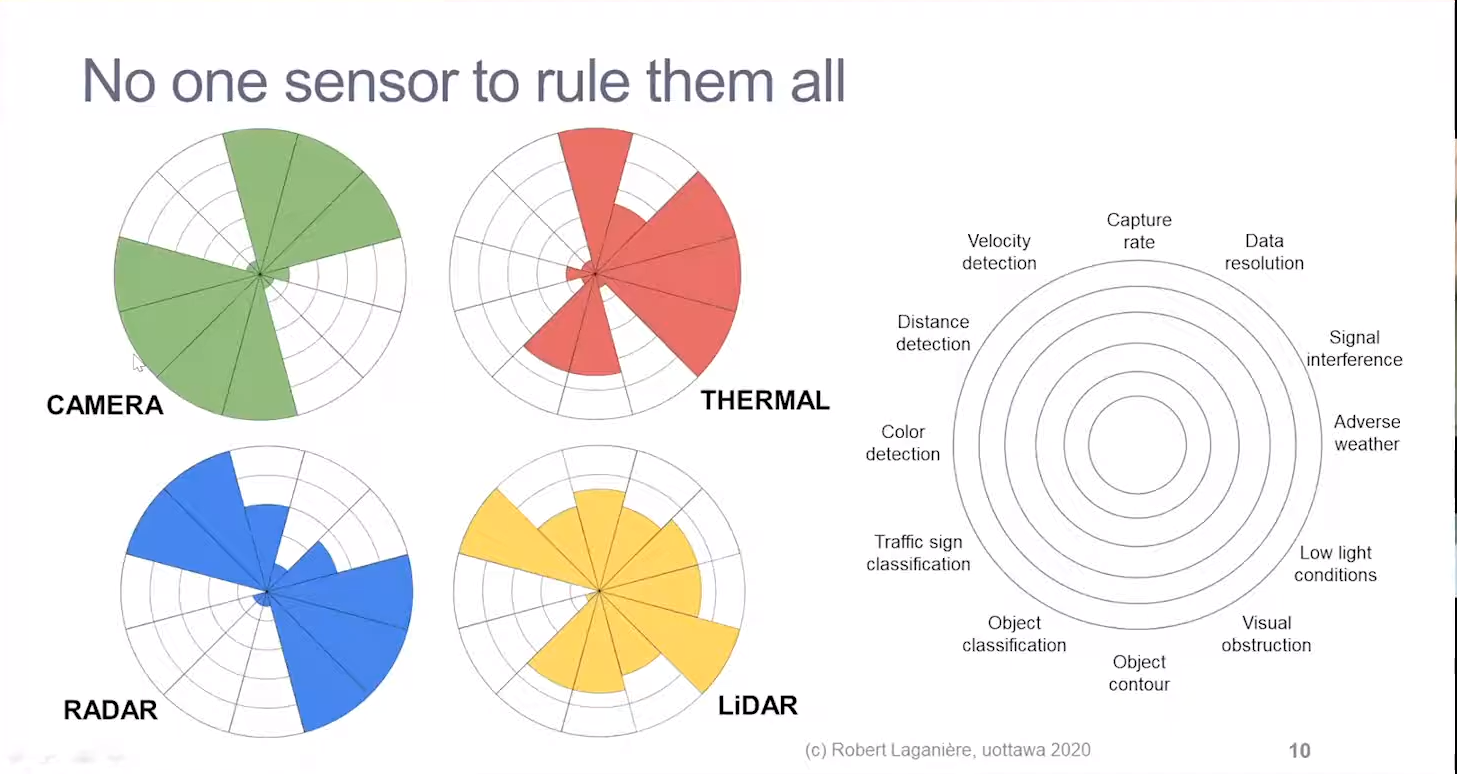
\includegraphics[width=0.7\textwidth]{images/sensors_intro_1.png}
                \caption{Sensors modality characteristics \cite{Sensor_modality_characteristics_1}}
                \label{fig:sensors_intro_1}
            \end{figure}

        \item To address these challenges, this project aims to implement a multimodal sensor fusion system that combines cameras, radar, and LiDAR sensors. By fusing data from multiple sensors and leveraging advanced machine learning algorithms, the goal is to enhance object detection's range, accuracy, and reliability in adverse weather conditions.
        
        \item The focus will also be on synchronizing multimodal data, processing dense and sparse resolution sensor data, and using a data-driven approach to optimize object detection performance.

            \begin{figure}[h]
                \centering
                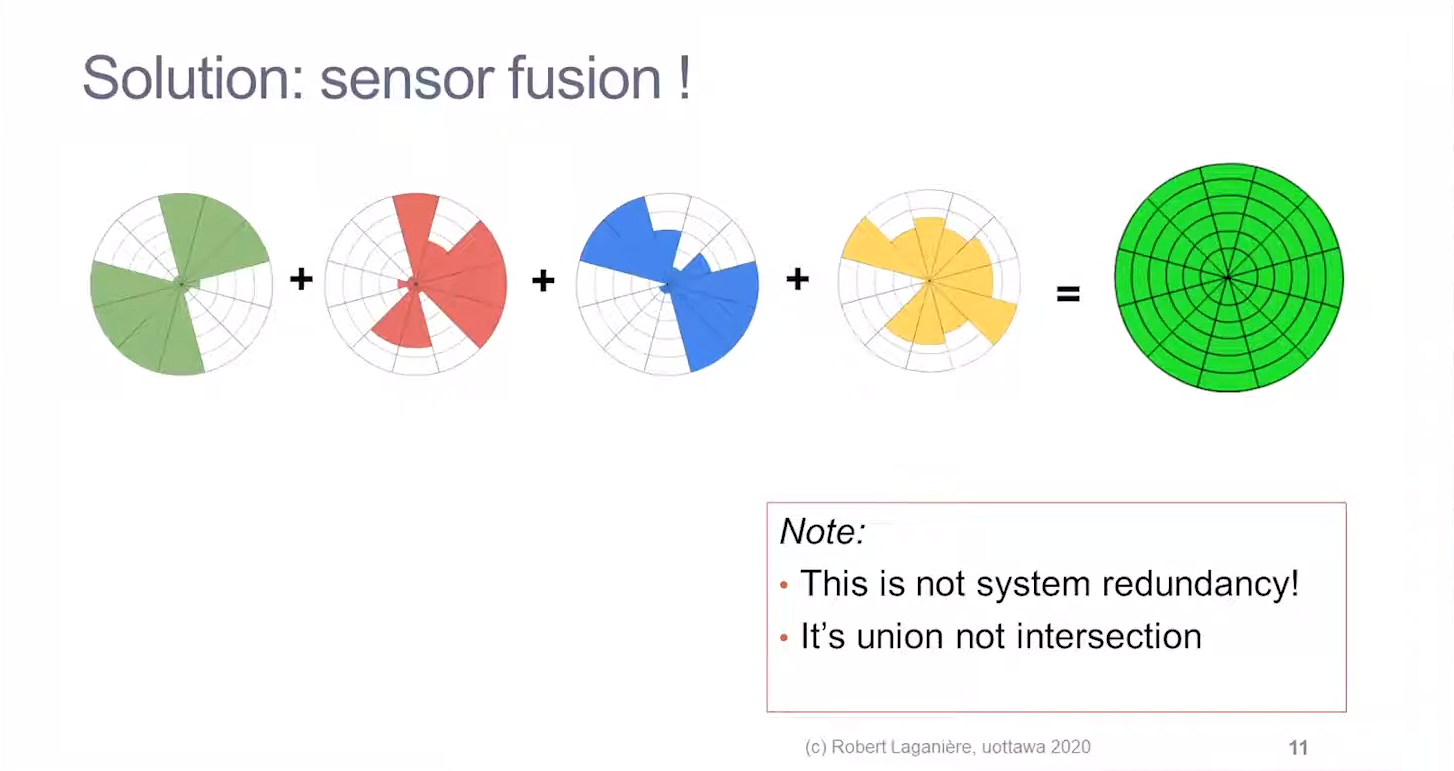
\includegraphics[width=0.7\textwidth]{images/sensors_intro_2.png}
                \caption{Sensors modality characteristics \cite{Sensor_modality_characteristics_1}}
                \label{fig:sensors_intro_2}
            \end{figure}

        \item However, this project also faces several challenges. For example, different sensors may have different resolutions, sampling rates, and may require sophisticated calibration and alignment techniques to ensure the accurate fusion of their data. Furthermore, processing large volumes of sensor data with minimal latency requires efficient and scalable algorithms and hardware architectures.

        \item The proposed system will be trained on a diverse dataset to ensure robustness and adaptability in different weather and lighting conditions. The system's effectiveness will be evaluated by extensive experiments and by comparing existing state-of-the-art methods.

        \item Despite the challenges, the project has the potential to revolutionize object detection in adverse weather conditions, with applications ranging from self-driving cars, drones to surveillance, and security systems. By fusing multiple sensor data sources and optimizing their fusion, situational awareness can be enhanced, enabling safer and more efficient operations in various domains.

        \item This research aims to facilitate safe and efficient self-driving in adverse weather conditions, prioritizing the safety of passengers, other drivers, and pedestrians on the road. To accomplish this, the proposed approach is to develop a sensor fusion system that operates with minimal latency, enabling data processing from multiple sensors in near real-time.
        \item Topic naming convention:
          \begin{itemize}
              \item Object detection
                    \begin{itemize}
                        \item Refers to the task of detecting objects within an image or video stream.
                        \item In this project, the focus is on detecting objects such as cars, trucks, pedestrians, and cyclists.
                    \end{itemize}
              \item Adverse weather conditions
                    \begin{itemize}
                        \item Refers to conditions such as fog, snow, rain, overcast skies, sleet, and dust.
                        \item These conditions can make object detection more challenging due to reduced visibility or other environmental factors.
                    \end{itemize}
              \item Tightly-coupled
                    \begin{itemize}
                        \item Refers to how different modalities of data are combined and integrated at different levels.
                        \item Rather than relying solely on early, mid, or late fusion techniques, a combination of features at different levels is employed to achieve optimal fusion results.
                    \end{itemize}
              \item Data-driven
                    \begin{itemize}
                        \item Refers to the use of previously collected data or publicly available datasets to improve object detection performance.
                    \end{itemize}
              \item Multimodal
                    \begin{itemize}
                        \item Refers to the use of different data modalities to improve object detection performance.
                        \item Examples include sensors such as camera, LIDAR, RADAR, IMU, GPS, and infrared, with different datatypes such as point clouds, images, and time series data.
                    \end{itemize}
              \item Sensor fusion
                    \begin{itemize}
                        \item Refers to the process of fusing data from different sensors to get a better estimation of an environment and improve object detection performance.
                    \end{itemize}
          \end{itemize}
    
    \end{itemize}
    \section{Relevance}

    \begin{itemize}

        \item The relevance of the research project lies in the fact that weather phenomena have a significant negative influence on traffic and transportation, which can lead to accidents, injuries, and fatalities.

        \item The statistics show that adverse weather conditions, such as rain, snow, sleet, and fog, contribute to a high number of vehicle crashes and fatalities worldwide.

        \item For example, in the United States, over 30,000 vehicle crashes occur on snowy or icy roads each year, causing over 5,000 fatalities and 418,000 injuries due to adverse weather-related crashes, according to the Federal Highway Administration (FHA) \cite{federal-highway-administration-no-date} \cite{usDepartmentofCommerce2016}.

        \item According to a study by the Insurance Institute for Highway Safety (IIHS), the likelihood of fatal crashes increases significantly during snowy weather conditions, with a 21\% higher rate compared to clear roads. The rate is even higher at 37\% during sleet and freezing rain. Furthermore, a report by the National Highway Traffic Safety Administration (NHTSA) in 2018 revealed that adverse weather conditions were involved in 4,000 fatal crashes \cite{brumbelow2022light}.

        \item In Europe, adverse weather conditions cause 25\% of all road accidents, with frost and ice, snow, and rain being the highest contributing factors, according to the European Commission and the European Transport Safety Council (ETSC). Over 12,000 people die on European roads each year in weather-related accidents \cite{cookson-2022}.

        \item Furthermore, the project's results will benefit various sectors, including autonomous vehicles, healthcare, precision agriculture, environmental monitoring, aerospace and defense, and industrial automation.
        
        \item In 2019, the global market for sensor fusion used in autonomous vehicles had a value of USD 594.4 million. According to estimates, this market is expected to grow significantly and reach a value of USD 1563.5 million by 2025, reflecting a Compound Annual Growth Rate (CAGR) of 19.6\% during the period between 2020 and 2025. According to MarketInsider, autonomous emergency braking (AEB) is expected to drive significant growth in the use of sensor fusion, as AEB systems rely on radar and vision sensors to identify potential collision partners ahead of the ego vehicle. North America is predicted to be one of the largest markets for ADAS-enabled vehicles and self-driven transport solutions \cite{marketInsider}.

        \item In the healthcare sector, wearable sensors are estimated to reach over \$1.5 billion in revenue by 2030, growing at a CAGR of over 18.3\% \cite{straitsresearch2021}.

        \item For precision agriculture and environmental monitoring, the market is expected to reach \$10.5 billion by 2026, growing at a CAGR of over 12.6\% \cite{mordorintelligence2023}.

        \item The aerospace and defense sector, including aircraft navigation and control, missile guidance, and military logistics, is expected to reach \$23.83 billion by 2027, at a CAGR of 4.21\% \cite{fortunebusinessinsights2023}.

        \item Even the industrial automation sector benefits from the sensor fusion technology as it can improve the efficiency of the production process and reduce the cost of production.
        
    \end{itemize}
    
    \section{Motivation}
    \subsection{...}

    \lipsum[6-10]

    \subsection{...}


    \section{Challenges and Difficulties}
    \subsection{...}

    \lipsum[11-15]

    \subsection{...}

    \subsection{...}



    \section{Problem Statement}
    \begin{itemize}
        \item Object detection using multiple modalities has become a topic of increasing interest in recent years. However, despite the wealth of research in this area, there is still a lack of comprehensive analysis and practical implementation of state-of-the-art methods under adverse weather conditions. Therefore, the primary objective of this research project is to provide a thorough analysis and practical implementation of state-of-the-art methods for object detection using multiple modalities, including but not limited to camera, LiDAR, and radar.

        \item One of the significant challenges in multimodal object detection is determining an appropriate fusion strategy to exploit the complementary characteristics of various sensors. For instance, fusing camera and 4D radar data is a critical research question that needs to be addressed. This research project will focus on identifying an optimal fusion strategy that leverages the strengths of each sensor while minimizing their weaknesses.
        \item This research project aims to conduct experiments to evaluate the performance of the proposed methods under adverse weather conditions. To achieve this, the outcomes will be compared with various models on recently released datasets such as K-radar \cite{Paek2022Jun}, DENSE \cite{bijelic2020seeing}, and aiMotive \cite{Matuszka2022Nov}. These datasets are deemed suitable for the purpose of analyzing the performance of the proposed methods under challenging conditions.
      
        \item The comparative analysis of the results will include an assessment of the strengths and weaknesses of each approach with respect to existing state-of-the-art methods.        

    \end{itemize}

    % \subsection{...}

    % \lipsum[21-30]

    % \subsection{...}


    % \subsection{...}
\end{document}
